\documentclass[../defence.tex]{subfiles}
\begin{document}

  \begin{frame}{Landauniveaus in Graphen II}
    \begin{columns}[onlytextwidth, T]
      \column{\dimexpr\linewidth / 3 * 2}
        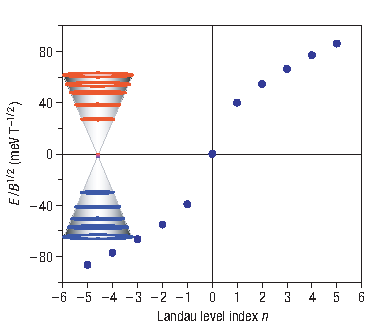
\includegraphics[width=\linewidth]{images/landau_dirac.pdf}
      \column{\dimexpr\linewidth / 3 * 2}
        \cite{li2007}
    \end{columns}
    \note{
    \begin{itemize}
      \item Keine Lücke zwischen Valenz- und Leitungsband
      \item Kegel statt Parabelförmigem Ding
      \item Wurzelverhalten zwischen den Landauniveaus, keine Äquidistanz
    \end{itemize}
    }
  \end{frame}

\end{document}
